\documentclass[11pt]{article}
\usepackage[margin=0.85in]{geometry}
\usepackage[T1]{fontenc}
\usepackage{lmodern,amsmath,amssymb,booktabs,tabularx,tikz,hyperref,xurl,float}
\usetikzlibrary{positioning,calc}
\hypersetup{colorlinks=true,linkcolor=blue!50!black,urlcolor=blue!50!black,citecolor=blue!50!black}
\definecolor{accent}{HTML}{3575B2}
\definecolor{warm}{HTML}{D1495B}
\tikzset{v/.style={circle,draw=accent,fill=white,thick,minimum size=6mm,inner sep=1pt},e/.style={thick,draw=gray!80},focus/.style={very thick,draw=warm}}
\newcommand{\N}{\mathcal N}
\newcommand{\R}{\mathcal R}
\newcommand{\eff}{r^{\mathrm{eff}}}
\newcommand{\plain}[1]{\noindent #1\par\smallskip}
\providecommand{\reportbuilddatetime}{unknown (standalone preview)}
\InputIfFileExists{graph_measures_build_info.tex}{}{}
\title{Edge and vertex measures for the SuiteSparse graph gallery}
\author{\parbox{0.94\linewidth}{\centering\small Source: \path{~/current_projects/gflowui/dev/suitesparse_project/graph_measures/graph_measures.tex}}}
\date{\small Build \reportbuilddatetime}
\begin{document}
\maketitle
\section{Purpose and scope}
A graph drawing can suggest a hub, a bottleneck, or a densely connected region. Which of these features belong to the graph itself, and which depend on where its vertices are drawn? This guide describes five edge measure families and five vertex measures that depend only on the saved graph. They distinguish immediate connectivity, short alternative routes, shortest-path traffic, and vulnerability to deleting one edge or vertex.

The definitions apply to the 80 selected SuiteSparse gallery graphs. Every edge has length one; the original matrix coefficients are not treated as distances. The figures are constructed examples: paths, cycles, triangles, stars and complete graphs chosen to isolate the meaning of each measure. Their values follow from the definitions, rather than from statistical estimation, so confidence intervals are not applicable. Higher values are not universally better: their meaning depends on the question and the construction of the graph.

The guide uses previously computed graph properties; building the report does not rerun those calculations. The saved property bundle and validation record are identified in Appendix~\ref{sec:reproduce}; the earlier computation did not record a result-generation timestamp. That missing timestamp is distinguished from the report build time shown above.

\clearpage
\section{The graph being measured}
Let $G=(V,E)$ be a simple undirected graph: there are no loops or repeated edges. Here $V$ is the vertex set and $E$ is the set of unordered vertex pairs that form edges. Write $n=|V|$ for the number of vertices, $m=|E|$ for the number of edges, and $\N(v)=\{u\in V:\{u,v\}\in E\}$ for the neighbors of vertex $v$; vertical bars denote set size. A connected component is a maximal set of mutually reachable vertices. Let $C(v)$ be the component of $v$, and $n_C=|C|$ the size of whichever component $C$ is under discussion. Define the adjacency matrix by
\[
 A_{uv}=\begin{cases}1,&\{u,v\}\in E,\\0,&\text{otherwise},\end{cases}\qquad u,v\in V.
\]
Thus $A$ records connections, with $A_{vv}=0$. Vertex labels have an arbitrary fixed order: $s<t$ means that each unordered pair is counted once. We use $\binom q2=q(q-1)/2$ for the number of unordered pairs among $q$ objects, and $\mathbf1\{S\}$ for the indicator of a statement $S$, equal to 1 when true and 0 otherwise. The complete graph $K_q$ joins every pair of its $q$ vertices.

The gallery gives every edge traversal length $\ell_e=1$. For distinct vertices $s,t$, let $\mathcal P_G(s,t)$ be the set of paths joining them. The shortest-path distance is
\[
 d_G(s,t)=\min_{P\in\mathcal P_G(s,t)}\sum_{e\in P}\ell_e,
\]
with $\min\varnothing=\infty$ and $d_G(s,s)=0$. For unit lengths this is the minimum number of edges in a path. Unreachable pairs have distance $\infty$ and contribute nothing to betweenness. The original matrix coefficients may be similarities, signed optimization weights, or equation coefficients; they are not used as lengths. All quantities refer to the \emph{saved gallery graph}, including any documented largest-component extraction, not automatically to the full source matrix.

\begin{table}[htbp]\centering\small\caption{The ten measure families and the questions they address. Each row names one family; the right column gives its interpretation. Definitions, units and exceptional cases follow in the corresponding sections.}\label{tab:measures}
\begin{tabularx}{\linewidth}{lX}
\toprule Edge property family & Question answered\\\midrule
Detour ratio & How much longer is the best alternative if this edge fails?\\
Edge betweenness & How much equal-demand shortest-path traffic uses it?\\
Triangle count & How many two-step alternatives connect its endpoints?\\
Effective resistance & How redundant is the connection when all routes can carry current?\\
Bridge and separation & Does deletion disconnect the graph, and how large is the split?\\\midrule
Vertex property & Question answered\\\midrule
Degree & How many immediate neighbors does it have?\\
Vertex betweenness & How much shortest-path traffic passes through it?\\
Core number & What minimum number of remaining neighbors can it retain under repeated pruning?\\
Local clustering & How often are pairs of its neighbors also connected?\\
Articulation point & Does deleting this vertex disconnect its component?\\\bottomrule
\end{tabularx}\end{table}
These are structural descriptions, not universal measures of scientific importance. Their interpretation depends on what vertices and edges mean in each dataset.

\clearpage
\section{Edge detour ratio}
\plain{The detour ratio compares the shortest replacement route with the length of the edge that was removed.}
For an edge $e=\{i,j\}$ with positive traversal length $\ell_e$, define
\begin{equation}
 R_e=\frac{d_{G-e}(i,j)}{\ell_e},\qquad G-e=(V,E\setminus\{e\}).
\end{equation}
Only the edge is deleted; its vertices remain. If the endpoints become disconnected, set $R_e=\infty$. In the gallery $\ell_e=1$, so $R_e$ is the alternate path's hop count. A finite value is at least 2. In a general positively weighted graph it can be below 1, if the direct edge is longer than an indirect route; that case does not occur here.

For unit lengths, $R_e+1$ is the length of the shortest cycle containing $e$. The proof is constructive: append $e$ to a shortest alternate path to form a cycle; conversely, remove $e$ from a shortest such cycle to obtain an alternate path. Thus triangles give detour 2, squares without a diagonal give detour 3, and bridges give infinity. In Figure~\ref{fig:detour}, remove the dashed edge in each of three separate graphs and count the edges in the remaining route between $i$ and $j$.
\par
\begin{figure}[H]\centering
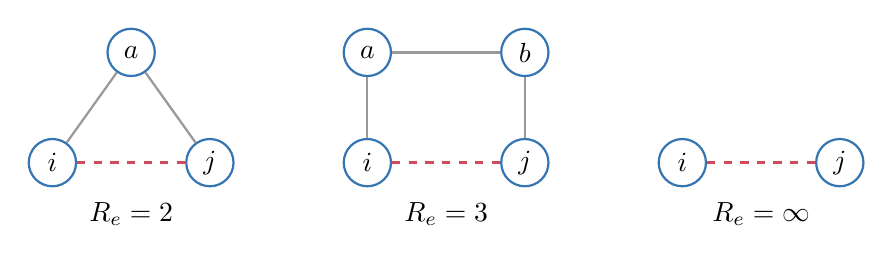
\begin{tikzpicture}[scale=1]
\begin{scope}
\node[v] (a) at (0,0) {$i$};\node[v] (b) at (2,0) {$j$};\node[v] (c) at (1,1.4) {$a$};
\draw[e] (a)--(c)--(b);\draw[focus,dashed] (a)--(b);
\node at (1,-.65) {$R_e=2$};
\end{scope}
\begin{scope}[xshift=4cm]
\node[v] (a) at (0,0) {$i$};\node[v] (b) at (2,0) {$j$};\node[v] (c) at (0,1.4) {$a$};\node[v] (d) at (2,1.4) {$b$};
\draw[e] (a)--(c)--(d)--(b);\draw[focus,dashed] (a)--(b);
\node at (1,-.65) {$R_e=3$};
\end{scope}
\begin{scope}[xshift=8cm]
\node[v] (a) at (0,0) {$i$};\node[v] (b) at (2,0) {$j$};
\draw[focus,dashed] (a)--(b);\node at (1,-.65) {$R_e=\infty$};
\end{scope}
\end{tikzpicture}
\caption{The dashed red edge is the edge being tested. The solid edges remain after deletion. Detour $R_e$ is 2 in the triangle, 3 in the square, and infinite for an isolated edge. These are three different graphs.}\label{fig:detour}
\end{figure}
\par
A large detour is useful for detecting a locally irreplaceable connection or a possible shortcut. It does not measure the total effect on all pairs, and an important legitimate long-range connection can have a large value. It also ignores how many equally good replacement routes exist.

\section{Edge triangle count}
\plain{Count the mutual neighbors that can connect the endpoints in two steps.}
\begin{equation}
 t_{ij}=|\N(i)\cap\N(j)|=\sum_{k\in V} A_{ik}A_{kj},\qquad \{i,j\}\in E,
\end{equation}
The sum runs over every possible common neighbor $k$. The count $t_{ij}$ is a nonnegative integer, measured in triangles. Each common neighbor completes exactly one triangle. In a complete graph on $q\geq3$ vertices, each edge has $q-2$ triangles, while its detour remains 2. Triangle count therefore distinguishes multiple short alternatives that detour cannot distinguish. Counts also depend on endpoint degree; zero is not by itself evidence of a bottleneck. Every edge in a bipartite graph has count zero, even when many longer cycles exist. The relation to vertex clustering is given in Section~\ref{sec:cluster}.

\clearpage
\section{Edge betweenness}
\plain{Imagine one unit of traffic between each reachable pair. Everyone uses shortest routes; tied routes share the traffic equally. Count the amount traversing each edge.}
Let $\sigma_{st}$ be the number of shortest paths from $s$ to $t$, and $\sigma_{st}(e)$ the number using $e$. With each unordered pair counted once,
\begin{equation}
 B_E(e)=\sum_{\substack{s<t\\s,t\in C(e)}}\frac{\sigma_{st}(e)}{\sigma_{st}},
 \qquad \widehat B_E(e)=\frac{B_E(e)}{\binom{n_C}{2}}.
\end{equation}
Here $C(e)$ is the component containing the edge. The endpoint pair $(i,j)$ is included. Raw betweenness is measured in units of routed pair demand; the normalized value is the expected share of one uniformly chosen component pair's unit demand using the edge. It lies between 0 and 1. This convention follows the undirected, fractional shortest-path definition, with a component-specific denominator~\cite{nxedge,brandes}. Figure~\ref{fig:traffic} isolates one pair before adding contributions from all pairs.
\par
\begin{figure}[H]\centering
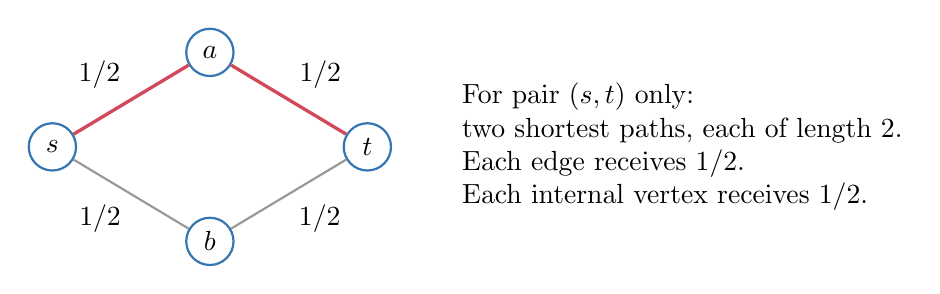
\begin{tikzpicture}
\node[v] (s) at (0,0) {$s$};\node[v] (a) at (2,1.2) {$a$};\node[v] (t) at (4,0) {$t$};\node[v] (b) at (2,-1.2) {$b$};
\draw[focus] (s)--node[above left] {$1/2$}(a)--node[above right] {$1/2$}(t);
\draw[e] (s)--node[below left] {$1/2$}(b)--node[below right] {$1/2$}(t);
\node[align=left] at (8,0) {For pair $(s,t)$ only:\\two shortest paths, each of length 2.\\Each edge receives $1/2$.\\Each internal vertex receives $1/2$.};
\end{tikzpicture}
\caption{Splitting credit avoids arbitrarily choosing one of two tied paths. In this four-cycle, summing all six unordered pairs gives $B_E=2$ for every edge. Vertex contributions will be defined in Section~\ref{sec:vertex-between}.}\label{fig:traffic}
\end{figure}
\par
For one edge of this square, its own endpoint pair contributes 1, and the two opposite-vertex pairs contribute $1/2$ each; all other pairs contribute zero. Hence $\widehat B_E=2/6=1/3$. This is a useful check against implementations that double-count directions.

The routing assumptions matter. Equal pair demand is a modeling choice, not a claim that every organism, equation, or physical junction sends the same traffic. Shortest-path routing is appropriate for some communication or distance models; it does not describe arbitrary diffusion or transport with capacity constraints. The manifold-shortcut paper uses betweenness to guide edge removal in neighborhood graphs~\cite{cukierski}. A high score can identify a candidate shortcut, but cannot establish that the original graph is erroneous.

Raw scores from components of different sizes are not directly comparable. Component normalization compares relative load \emph{within} each component; it does not make a tiny component equally consequential to the whole dataset. Both versions are retained. All gallery scores describe the original saved topology; selecting a different embedding or coloring mode never removes edges or recomputes a divisive sequence.

\clearpage
\section{Effective resistance of an edge}
\plain{Replace each edge by a unit resistor. Send one unit of current into one endpoint and remove it at the other. The required voltage difference measures how hard it is to connect the endpoints through all available routes.}
Let $L=D-A$ be the graph Laplacian, where $D$ is diagonal with $D_{ii}=\sum_{u\in V}A_{iu}$, the number of neighbors of $i$. For endpoints in the same component, write $b_{ij}=\mathbf e_i-\mathbf e_j$, where $\mathbf e_i$ has a 1 at position $i$ and zeros elsewhere. This vector describes unit current entering at $i$ and leaving at $j$. Then
\begin{equation}
 \eff_{ij}=b_{ij}^{\mathsf T} L^{+}b_{ij},
\end{equation}
Here the superscript $\mathsf T$ transposes a column vector. The matrix $L^{+}$ is the Moore--Penrose pseudoinverse, which inverts $L$ on its nonzero eigenspaces and assigns zero to its zero eigenspace. Equivalently, solve $Lx=b_{ij}$ after setting one vertex voltage to zero (grounding it), and take the voltage difference $x_i-x_j$. With unit current and one-ohm edge resistors, resistance is measured in ohms. The gallery computes this value for existing edges only, so no formula is applied across disconnected components. Effective resistance and its role in spectral sparsification are developed by Spielman and Srivastava~\cite{spielman}. The triangle below shows how current splits between a direct edge and a longer route.
\par
\begin{figure}[H]\centering
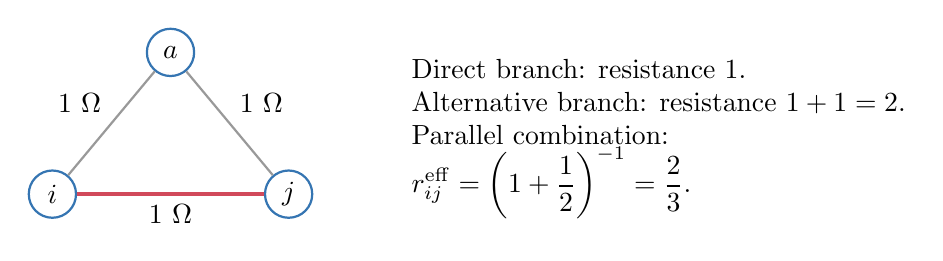
\begin{tikzpicture}
\node[v] (i) at (0,0) {$i$};\node[v] (j) at (3,0) {$j$};\node[v] (a) at (1.5,1.8) {$a$};
\draw[focus] (i)--node[below] {$1\ \Omega$}(j);
\draw[e] (i)--node[above left] {$1\ \Omega$}(a)--node[above right] {$1\ \Omega$}(j);
\node[align=left] at (7.7,.7) {Direct branch: resistance 1.\\Alternative branch: resistance $1+1=2$.\\Parallel combination:\\$\displaystyle \eff_{ij}=\left(1+\frac12\right)^{-1}=\frac23$.};
\end{tikzpicture}
\caption{A triangle has detour 2 but effective resistance $2/3$. Current can use the direct edge and the two-edge route simultaneously. These are mathematical unit resistors, not measured electrical properties of the dataset.}
\end{figure}
\par
The unit direct edge ensures $0<\eff_e\leq1$. A bridge has value 1 because there is no alternate conducting path between its endpoints. If an alternative exists, current can split and the value is strictly below 1. Thus smaller values indicate greater electrical redundancy; larger values indicate greater dependence on the connection.

For the triangle the value is $2/3$; for an edge of a four-cycle it is $3/4$; for an edge of the complete graph $K_q$ it is $2/q$. For $q\geq3$, all $K_q$ edges have detour 2, so resistance distinguishes global redundancy beyond the shortest replacement path. Unlike betweenness, current is not confined to shortest paths.

A spanning tree connects every vertex of a component without cycles. For unit conductances, $\eff_e$ also equals the probability that a uniformly random spanning tree of the component contains $e$~\cite{spielman}. Consequently,
\begin{equation}
 \sum_{e\in E}\eff_e=n-c,
\end{equation}
where $c$ is the number of components, including isolated vertices: take the expected number of edges in one spanning tree per component. This identity is checked during computation.

For positive weighted electrical networks, let $c_e>0$ denote conductance, the reciprocal of edge resistance. Then $L=\sum_{e=\{i,j\}\in E}c_e b_{ij}b_{ij}^{\mathsf T}$. Conductance is \emph{not} a shortest-path length. Restoring arbitrary signed source coefficients to this formula would be invalid. The implemented unit-resistor interpretation avoids that ambiguity.

\clearpage
\section{Bridge status and separation size}
\plain{A bridge is a single connection whose loss splits its component. Record how large the two resulting pieces are.}
Let $c(G)$ count connected components, including isolates. Define
\begin{equation}
 b_e=\mathbf 1\{c(G-e)>c(G)\}.
\end{equation}
This is the standard bridge definition~\cite{nxbridge}. The indicator $b_e$ is 1 for a bridge and 0 otherwise. For a bridge in a component of size $n_C$, deletion produces sets of sizes $a$ and $n_C-a$. Define
\begin{equation}
 s_e=\min(a,n_C-a),\quad l_e=\max(a,n_C-a),\quad P_e=s_e l_e.
\end{equation}
Here $s_e$ and $l_e$ count vertices in the smaller and larger pieces, respectively. Exactly $P_e$ unordered vertex pairs lose connectivity. Every path between the two sides uses the bridge, so $B_E(e)=P_e$. The gallery checks this identity. For nonbridges, side sizes are \emph{not applicable}, while $P_e=0$ because no previously connected pair becomes disconnected. The path below compares all three possible single-edge deletions; $a\mid(n_C-a)$ labels the resulting piece sizes.
\par
\begin{figure}[H]\centering
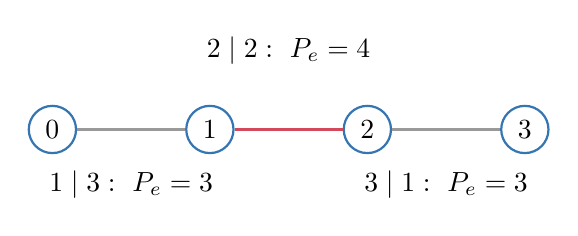
\begin{tikzpicture}
\foreach \i in {0,1,2,3}{\node[v] (p\i) at (2*\i,0) {$\i$};}
\draw[e] (p0)--(p1);\draw[focus] (p1)--(p2);\draw[e] (p2)--(p3);
\node at (1,-.7) {$1\mid3:\ P_e=3$};\node at (3,1) {$2\mid2:\ P_e=4$};\node at (5,-.7) {$3\mid1:\ P_e=3$};
\end{tikzpicture}
\caption{All three path edges are bridges and have infinite detour and unit effective resistance. Separation size distinguishes the central bridge, whose deletion separates four pairs, from either end edge, whose deletion separates three.}
\end{figure}
\par
This measure assumes a single edge failure. It says nothing directly about capacity, failure probability, or resilience to multiple simultaneous failures. Infinite detour alone should therefore not determine a ranking of bridge importance.

\clearpage
\section{Articulation-point status}
\plain{An articulation point is a vertex whose removal, together with its incident edges, splits its component into multiple pieces.}
\begin{equation}
 a_v=\mathbf 1\{c(G-v)>c(G)\}.
\end{equation}
Here $G-v$ removes $v$ and every incident edge. The indicator $a_v$ equals 1 for an articulation point and 0 otherwise~\cite{nxarticulation}. An isolated vertex or a leaf is not an articulation point. In the four-vertex path above, vertices 1 and 2 are articulation points. In two triangles sharing one vertex, the shared vertex is an articulation point although there are \emph{no bridges}: every edge still belongs to a cycle.
\par
\begin{figure}[H]\centering
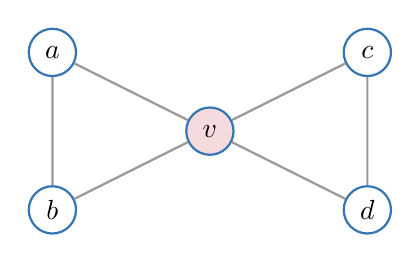
\begin{tikzpicture}
\node[v,fill=warm!20] (o) at (0,0) {$v$};
\node[v] (a) at (-2,1) {$a$};\node[v] (b) at (-2,-1) {$b$};
\node[v] (c) at (2,1) {$c$};\node[v] (d) at (2,-1) {$d$};
\draw[e] (o)--(a)--(b)--(o)--(c)--(d)--(o);
\end{tikzpicture}
\caption{Deleting $v$ splits this graph into two edges. Deleting any single edge leaves the graph connected. Vertex failure and edge failure expose different vulnerabilities.}
\end{figure}
\par

\clearpage
\section{Vertex degree}
\plain{Count the immediate neighbors.}
\begin{equation}
 d_v=\deg(v)=|\N(v)|=\sum_{u\in V} A_{vu}.
\end{equation}
Degree is a local baseline. Zero identifies an isolate; one identifies a leaf. A high value can mean many direct interactions, many coupled variables, or many nearby observations, depending on graph construction. It is not automatically a measure of influence or centrality in the full network. In particular, a graph that joins each observation to its $k$ nearest neighbors and then ignores edge direction can have degrees above $k$, because other observations can select it too; $k$ is the chosen number of neighbors per observation.

\section{Vertex core number}
\plain{Core number measures how many neighbors a vertex can retain when vertices with too few remaining neighbors are repeatedly removed.}
For each integer $k\geq0$, let $H_k$ be the maximal induced subgraph of $G$ in which every vertex has degree at least $k$ \emph{within that subgraph}. Define
\begin{equation}
 \kappa(v)=\max\{k\geq0:v\in V(H_k)\}.
\end{equation}
An induced subgraph retains all original edges between its retained vertices, and $V(H_k)$ is its vertex set. Thus $\kappa(v)$ is the largest integer minimum-degree threshold that $v$ can survive. The $k$-core is obtained by repeatedly deleting vertices of current degree less than $k$. This definition and a linear-time implementation are given by Batagelj and Zaver\v{s}nik~\cite{cores}. Core number is at most degree. Isolates have core number zero; every vertex of a nontrivial tree has core number one, including its highest-degree hub. A cycle has core number two everywhere, and $K_q$ has core number $q-1$. The figure compares a five-leaf star with $K_4$: focus on the labeled vertex $v$ in each graph.
\par
\begin{figure}[H]\centering
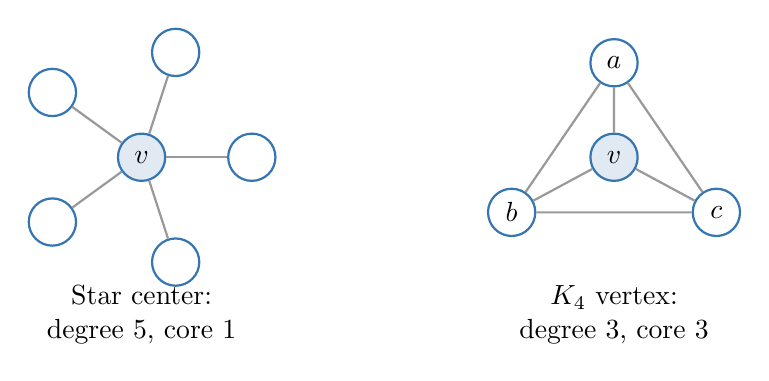
\begin{tikzpicture}
\node[v,fill=accent!15] (o) at (0,0) {$v$};
\foreach \i/\ang in {1/0,2/72,3/144,4/216,5/288}{\node[v] (s\i) at (\ang:1.4) {};\draw[e] (o)--(s\i);}
\node[align=center] at (0,-2) {Star center:\\degree 5, core 1};
\begin{scope}[xshift=6cm]
\node[v] (a) at (0,1.2) {$a$};\node[v] (b) at (-1.3,-.7) {$b$};\node[v] (c) at (1.3,-.7) {$c$};\node[v,fill=accent!15] (d) at (0,0) {$v$};
\draw[e] (a)--(b)--(c)--(a);\draw[e] (d)--(a) (d)--(b) (d)--(c);
\node[align=center] at (0,-2) {$K_4$ vertex:\\degree 3, core 3};
\end{scope}
\end{tikzpicture}
\caption{A high-degree star center depends entirely on leaves. Once leaves are removed, it has no support. The lower-degree vertex in $K_4$ belongs to a mutually connected group that survives a minimum-degree threshold of 3.}
\end{figure}
\par
Coreness is useful when recursive structural support matters. It neither identifies a unique community nor guarantees short paths between all members. A $k$-core can be disconnected and need not resemble a clique. Regular meshes may give almost constant core values despite visually distinctive geometry.

\clearpage
\section{Vertex betweenness}\label{sec:vertex-between}
\plain{Using the same equal-demand routing model as edge betweenness, count traffic passing through a vertex rather than starting or ending there.}
For $v\in C$, define
\begin{equation}
 B_V(v)=\sum_{\substack{s<t;\ s,t\in C\setminus\{v\}}}
 \frac{\sigma_{st}(v)}{\sigma_{st}},\qquad
 \widehat B_V(v)=\begin{cases}
 B_V(v)/\binom{n_C-1}{2},&n_C\geq3,\\0,&n_C<3.
 \end{cases}
\end{equation}
Here $\sigma_{st}(v)$ counts shortest paths on which $v$ is an \emph{internal} vertex. This endpoint convention is explicit in the standard implementation~\cite{nxvertex}. In a star with $q$ leaves, the center has $B_V=\binom q2$ and normalized value 1; all leaves have value zero. In $K_q$, every vertex has betweenness zero because each pair is joined directly. High degree therefore need not imply high betweenness.

Raw $B_V$ has units of routed pair demand; $\widehat B_V$ is dimensionless and lies between 0 and 1. Its denominator counts possible endpoint pairs after excluding $v$. The zero convention for components smaller than three vertices avoids division by zero. For the four-cycle in Figure~\ref{fig:traffic}, each vertex gets $1/2$ from the pair of its two neighbors. Its normalized score is $(1/2)/3=1/6$. A vertex can have positive betweenness without being an articulation point: alternative longer paths can preserve connectivity even when shortest traffic prefers that vertex.

\section{Local clustering coefficient}\label{sec:cluster}
\plain{Local clustering is the fraction of pairs of a vertex's neighbors that are themselves connected.}
Let $T_v$ count triangles containing $v$. Then
\begin{equation}
 C_v=\begin{cases}\displaystyle\frac{T_v}{\binom{d_v}{2}}
 =\frac{2T_v}{d_v(d_v-1)},&d_v\geq2,\\0,&d_v<2.
 \end{cases}
 \qquad T_v=\frac12\sum_{u\in\N(v)}t_{uv}.
\end{equation}
The convention $C_v=0$ for fewer than two neighbors assigns a value when there are no possible neighbor pairs~\cite{nxcluster}. Each triangle containing $v$ contributes to two incident edge triangle counts, explaining the factor $1/2$. The dimensionless fraction $C_v$ lies between 0 and 1; larger values mean more connections among neighbors. In the figure, compare the one existing neighbor-to-neighbor edge with the three possible pairs.
\par
\begin{figure}[H]\centering
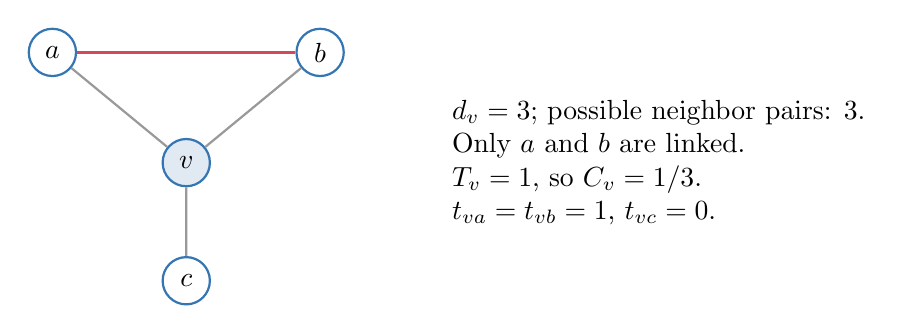
\begin{tikzpicture}
\node[v,fill=accent!15] (v) at (0,0) {$v$};
\node[v] (a) at (-1.7,1.4) {$a$};\node[v] (b) at (1.7,1.4) {$b$};\node[v] (c) at (0,-1.5) {$c$};
\draw[e] (v)--(a) (v)--(b) (v)--(c);\draw[focus] (a)--(b);
\node[align=left] at (6,0) {$d_v=3$; possible neighbor pairs: 3.\\Only $a$ and $b$ are linked.\\$T_v=1$, so $C_v=1/3$.\\$t_{va}=t_{vb}=1$, $t_{vc}=0$.};
\end{tikzpicture}
\caption{Clustering normalizes triangle abundance by the number of opportunities. The leaf $c$ is an example where the assigned clustering value is zero because degree is below two.}
\end{figure}
\par
Local clustering quantifies triangular closure; it does not directly measure density at larger distances. All bipartite graphs have $C_v=0$, including dense complete bipartite graphs. Conversely, high local clustering can coexist with a bridge joining two dense regions. This makes clustering complementary to both betweenness and bridge status.

\clearpage
\section{Using the gallery controls}
Vertex color can encode degree, raw or component-normalized betweenness, core number, clustering, or articulation status. Edge color can encode detour ratio, raw or normalized betweenness, triangle count, resistance, bridge status, either bridge-side size, or the number of separated pairs. The extra bridge fields belong to one property family, not additional independent centralities.

Continuous structural colors run from purple (low) through green to yellow (high), using the selected graph's range. The scale therefore stays fixed when the embedding changes; identical colors across different graphs need not mean identical numbers. A red edge indicates an infinite detour, and gray indicates an inapplicable bridge-side size. Neither is silently mapped to a large finite number or to zero. Numeric colorbars and hover values provide the actual scale. The existing drawn-length coloring remains layout-dependent and distinct from these structural measures.

Vertex labels can show IDs or IDs with a chosen property, for selected vertices or all vertices. Edge labels show a chosen property at edge midpoints, either for all edges or for edges touching selected vertices. Dense graphs are more readable with restricted labels; midpoint hover exposes edge values without labeling everything. Selection is indicated separately from the property's color.

These controls support inspection, not automatic pruning. A meaningful next analysis might compare large detours with high betweenness and high resistance, while retaining bridges as a separate category. Agreement identifies edges worth examining in the context of the graph's construction; it does not prove that those edges are spurious.

\clearpage
\appendix
\section{Computation and reproducibility}\label{sec:reproduce}
The report build time is \reportbuilddatetime. Calculations are reused from the saved property bundle; rebuilding this document does not recompute graph measures. The bundle does not contain a recorded generation timestamp, so its exact generation time cannot be recovered from its contents. File modification times are not substituted for that missing record.

The exact property index is \href{file:///Users/pgajer/current_projects/suitesparse_embedding_comparison/graph_properties/ca5c83e2d2e9db7a9f41c234c1694c4d76911279acec9adb2a566db23e4f3982.json}{the saved property manifest}; its content hash is
\begin{quote}\small\path{ca5c83e2d2e9db7a9f41c234c1694c4d76911279acec9adb2a566db23e4f3982}.\end{quote}
The \href{file:///Users/pgajer/current_projects/suitesparse_embedding_comparison/graph_measures_30_sept_2026/validation.json}{validation record} covers all 80 gallery graphs, containing 52,913 vertices and 334,278 edges; no gallery graph is excluded. The calculations are deterministic and use no random source sampling. The figures in this guide are vector drawings defined directly in the LaTeX source.

\subsection{Algorithms and checks}
The implementation preserves the graph's exact vertex order and edge order. Properties are stored with graph and file checksums. Selecting a different embedding does not change them. Component-normalized betweenness uses the component sizes in the graph actually displayed; an extracted component is analyzed in its own right.

Degree uses adjacency lists. Triangle counts use intersections of neighbor sets. Vertex clustering follows from the incident triangle counts. Bridges and articulation points use graph traversal; core numbers use recursive degree pruning. Betweenness uses all-source shortest-path accumulation, rather than enumerating all shortest paths or sampling source vertices~\cite{brandes}. The detour search skips the tested edge, stops when the other endpoint is reached, and uses known triangle and bridge cases directly.

Effective resistance uses a grounded Laplacian factorization for each component. If vertex $r$ is grounded, invert $L$ with row and column $r$ removed, then pad the inverse by a zero row and column at $r$. Calling this padded matrix $Q$,
\begin{equation}
 \eff_{ij}=Q_{ii}+Q_{jj}-2Q_{ij}.
\end{equation}
The result is independent of which vertex was grounded. Floating-point linear algebra produces numerical values, not symbolic fractions; no stochastic resistance approximation is used. The implementation checks resistance bounds and the sum identity $\sum_e\eff_e=n-c$.

Small-graph tests independently enumerate all shortest paths and split credit, compare edge-deleted path lengths, and compare resistance with an independent pseudoinverse calculation. Fixtures include paths, cycles, complete graphs, stars, bipartite graphs, shared-vertex triangles, disconnected graphs, and isolates. In particular, the four-cycle tests tied paths rather than just unique routing. Bridge pair counts are checked against edge betweenness for every gallery graph.


\subsection{Reproduction commands and evidence}
From the gflowui repository, the calculation command is
\begin{quote}\small\ttfamily
python dev/suitesparse\_project/compute\_graph\_properties.py DATA\_ROOT --workers 4
\end{quote}
Here \texttt{DATA\_ROOT} is \path{~/current_projects/suitesparse_embedding_comparison}; use the gallery Python environment described in the pipeline README. The saved bundle records NetworkX 3.7, NumPy 2.5.3 and SciPy 1.18.1. From the report source directory, \texttt{make pdf} refreshes the generated build metadata and compiles the PDF; \texttt{make citation-check} checks the existing citation evidence against the compiled log. The \href{file:///Users/pgajer/current_projects/gflowui/dev/suitesparse_project/graph_measures/citation_verification.html}{citation verification record} links each scholarly claim to its source. The standalone editor can preview the source without auxiliary files; its fallback explicitly reports an unknown build timestamp if the generated metadata file is unavailable.

\clearpage
\begin{thebibliography}{9}
\bibitem{cukierski} W.~J. Cukierski and D.~J. Foran. Using Betweenness Centrality to Identify Manifold Shortcuts. \emph{IEEE International Conference on Data Mining Workshops}, 949--958, 2008. \href{https://doi.org/10.1109/ICDMW.2008.39}{doi:10.1109/ICDMW.2008.39}. \href{https://pmc.ncbi.nlm.nih.gov/articles/PMC2895570/}{Open manuscript}.
\bibitem{brandes} U. Brandes. A Faster Algorithm for Betweenness Centrality. \emph{Journal of Mathematical Sociology}, 25(2):163--177, 2001. \href{https://doi.org/10.1080/0022250X.2001.9990249}{doi:10.1080/0022250X.2001.9990249}.
\bibitem{spielman} D.~A. Spielman and N. Srivastava. Graph Sparsification by Effective Resistances. \emph{SIAM Journal on Computing}, 40(6):1913--1926, 2011. \href{https://doi.org/10.1137/080734029}{doi:10.1137/080734029}. \href{https://arxiv.org/abs/0803.0929}{Author preprint}.
\bibitem{cores} V. Batagelj and M. Zaver\v{s}nik. An $O(m)$ Algorithm for Cores Decomposition of Networks. Preprint, 2003. \href{https://arxiv.org/abs/cs/0310049}{arXiv:cs/0310049}.
\bibitem{nxedge} NetworkX Developers. \emph{Edge betweenness centrality}, documentation, accessed 30 September 2026. \url{https://networkx.org/documentation/stable/reference/algorithms/generated/networkx.algorithms.centrality.edge_betweenness_centrality.html}.
\bibitem{nxvertex} NetworkX Developers. \emph{Vertex betweenness centrality}, documentation, accessed 30 September 2026. \url{https://networkx.org/documentation/stable/reference/algorithms/generated/networkx.algorithms.centrality.betweenness_centrality.html}.
\bibitem{nxcluster} NetworkX Developers. \emph{Clustering}, documentation, accessed 30 September 2026. \url{https://networkx.org/documentation/stable/reference/algorithms/generated/networkx.algorithms.cluster.clustering.html}.
\bibitem{nxbridge} NetworkX Developers. \emph{Bridges}, documentation, accessed 30 September 2026. \url{https://networkx.org/documentation/stable/reference/algorithms/generated/networkx.algorithms.bridges.bridges.html}.
\bibitem{nxarticulation} NetworkX Developers. \emph{Articulation points}, documentation, accessed 30 September 2026. \url{https://networkx.org/documentation/stable/reference/algorithms/generated/networkx.algorithms.components.articulation_points.html}.
\end{thebibliography}
\end{document}
